
{\small
{\bf These bullets summarize the flow of the text (to be deleted in the final edit):
\begin{itemize}
\item  A New vision of ``institutional controls''.
\item  Personal data as the driver for current digital economies and future digital institutions.
\item  The role of Computational Law.
\item  Defining Controls for Digital Institutions in terms of Trust Networks.
\item  The New Digital Institution Stack
\item  Digital Institutions that Self-Control: the Vision
\end{itemize}
(The text below is REV05 -- \today)
}
}
~~\\


The Internet offers a new opportunities for individuals,
communities and societies to interact based on 
self-organized governance.
Currently there is arguably an inequitable access to resources
on the Internet -- including to ``personal data'' -- 
where incumbent service providers
and digital technology providers seek to resist
open network dynamics and to maintain the old business models
which in the long term benefit only a fraction 
of the Internet population~\cite{greene2008reality,pentland2009reality,WEF2011}.
Current social networking platforms typically
rely upon proprietary business models that collect and sell
personal information about users,
inducing social distrust in these business models~\cite{HardjonoDeegan2014}.

The World Economic Forum has identified personal data
as a new asset class~\cite{WEF2011} upon which new forms of future
economic activities may develop.
In order for for data to attain its true potential in the future
global digital economy, new forms of {\em digital communities}
must be allowed to flourish and evolve over time.
Similar to communities that over time evolved into institutions that we know today 
(e.g. New York Stock \& Exchange Board from the early 1800's),
digital communities within the virtual space on the Internet
must be recognized as having a legitimate role in the global economy
and be permitted to evolve unhindered into 
future {\em digital institutions}~\cite{Clippinger2013-InternetDisruption}.

Self-governance of digital communities is an important
ingredient for these communities to develop into
digital institutions. 
In the work of~\cite{Clippinger2013-InternetDisruption}
the notion of self-governance means the use
of data access policies and data usage policies
that are implemented as {\em computational law},
where governance is built into the computational engines
that are part-and-parcel of the technologcal infrastructure
which implements the virtual community.


If personal data is to be considered as
a new assets class~\cite{WEF2011}
then there is a need for a new paradigm for considering
the role and importance of personal data in 
the world's digital institutions and digital economy of the future.
Correspondingly, for these emerging digital institutions
there needs to be a new paradigm for contemplating
the aspects of ``institutional control'' within these
future institutions.






\subsection{Personal Data Assets as the Foundation for Future Digital Institutions}

The promise of the economic benefits from equal access to 
data -- personal data, proprietary data, and government data --
is difficult to argue against.
Today an example of a revolutionary use of data
as the basis for new forms of economic activities
can be found in {\em virtual currencies} as exemplified
by systems such as {\em BitCoin}~\cite{BarberBoyen2012} and
{\em Ven}~\cite{Stalnaker2013}.
Like their brick-and-mortar equivalents,
these virtual currency systems can flourish
only if all the system participants have equal access
to data, be it market data, meta-data about the system itself,
provenance information regarding certain data,
or data that are used as assets to back certain currencies.
Just as inequitable access to market data today results
in an inefficient economic system,
the inequitable access to data on the Internet
-- including personal data that forms the basis for market data --
results in inefficient digital institutions.

The economic benefits derived from the availability of data
describing attributes of individuals (i.e. private information)
and data capturing the behavior of individuals is undeniable.
For example, the online consumer buying behavior now drives much
of the selling plans occurring at different seasons
of the annual retail market.
Similarly, one can argue that in the large social networks (e.g. Facebook)
the individual user is seen not a customer but rather as the product itself.
Thus, artificially divorcing the role
of an individual's data (as an asset form) from its economic role
(and therefore from its legal role) is short-sighted,
and subsequently denies the full potential of personal data
as an engine of the new global digital economy.


We also need a new paradigm for considering future digital institutions,
and aspects of their roles and responsibilities to their
stakeholders and to society at large.
This new paradigm must enable nascent digital institutions
(such as the virtual currency systems of today)
to consider the more subtle notions related to personal data
in the larger context of social interactions on the Internet.
Thus, in defining future ``institutional controls''
in the digital economy, digital institutions must embrace
the notions of the {\em provenance} of data,
of {\em ownership} of data (beyond copyright),
of {\em common-pool sharing} of  data within and across digital institutions,
of {\em self-governance} of digital institutions
and the use of artificial intelligence and machine learning
to effect computational law.

This new paradigm must accommodate the notion of personal data as 
common-pool resource~\cite{Ostrom2009} on an opt-in basis.
The foundational concept of the common-pool resource
was put forward by  Elinor Ostrom, the Nobel Laureate in
economics in 2009.
Ostrom identified key principles by which 
self-organized groups can manage common-pool resources in fair, 
sustainable ways.  
If data were to be regarded as a common-pool resource, 
Ostrom’s research shows how it would be possible 
for online groups to devise their own {\em data commons} 
to manage their personal data in their own interests.
This open the possibility for the data commons to be
the basis of self-organizing digital institutions,
where ``law'' would have a very different character from
the kinds law we know today.
The development of `` digital law'' or computational law
in self-organizing digital institutions
would enable users to devise new types
of legal contracts that are
computationally expressible and 
executable~\cite{HardjonoDeegan2014,Clippinger2013-InternetDisruption}.



\subsection{Trust Networks as the Legal Foundation of Digital Institutions}

A promising model for self-governing digital institutions based on computational law
is that of {\em Trust Networks}.
In simple terms, a trust network for digital communities represents
the community rules and operational regulations which all members
of the community are bound to from they time they opt-in into membership
of the community.

In the current brick-and-mortar economy there are a number of examples
of ``networks of trust'' that allow communities to pool resources and share risks.
In the international banking community the emergence
of the SWIFT network~\cite{SWIFTnetwork} 
(Society for Worldwide Interbank Financial Telecommunication) 
in the 1970s represented a major milestone for global banking.
The SWIFT network established a secure and reliable electronic network
that enables enables financial institutions worldwide 
to send and receive information about financial transactions.
Banks and financial institutions who wish to make use of the SWIFT network
must join the network by accepting a membership agreement.

Similarly, various identity federation consortium or organizations
have been established in the recent past with the aim of providing
a legal foundation to the creation, use and disposal of digital identities
on the Internet.
A recent example of such an organization is
the {\em Open Identity Exchange}~\cite{OIX-website}
whose aim is to create a {\em  Trust Framework} for identity federation
on the Internet
In digital identity systems, a trust framework
is a certification program that enables a party
who accepts a digital identity credential
(called the relying party) to trust the identity,
security, and privacy policies of the party
who issues the credential (called the identity
service provider) and vice versa~\cite{OIX-website}.

Currently efforts on legal ``trust frameworks''
are focused primarily on individual identity and identity federation.
However, we believe that a new legal foundation is
required for the personal data ecosystem and for
the various digital institutions that may utilize
personal data.
We believe a new view of the ``Internet stack''
needs to be introduced, where the stack
calls-out and recognizes the importance of personal data
and the crucial role of personal data stores or accounts.



\begin{figure*}[!t]
\centering
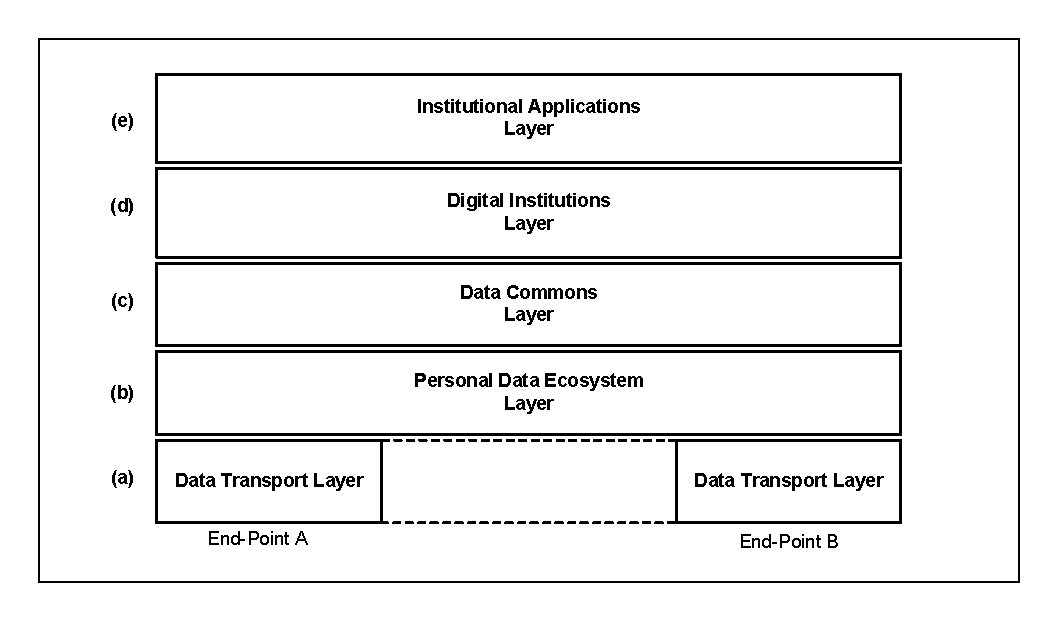
\includegraphics[width=7in]{figure-new-stack}
% where an .eps filename suffix will be assumed under latex, 
% and a .pdf suffix will be assumed for pdflatex; or what has been declared
% via \DeclareGraphicsExtensions.
\caption{A New Stack for Digital Institutions (after~\cite{HardjonoDeegan2014})}
\label{fig:newstack}
\end{figure*}



\subsection{Digital Institutions: A New Stack for the Internet}

In order for society to obtain the benefits of 
personal data as a the new asset class,
a new personal data ecosystem must evolve where
every stakeholder has equitable access to data and other resources
within the ecosystem.
Such equitable access must be available not only to individuals
real-world communities,
but also to emerging digital communities and institutions.

We believe that a new vision is needed for seeing the 
Internet, personal data and digital institutions
in a consistent manner, something akin to the Internet
TCP/IP stack or the 7-layer ISO stack\footnote{
The network engineering view of the Internet sees
in in a 4-layer view, whereas the International standards
perceives the Internet consisting of 7 layers.
In reality these view converge on the core functions
of necessary for the Internet to function today.}.
Such a stack -- termed the {\em digital institution stack} in~\cite{HardjonoDeegan2014} --
would be useful for viewing the evolving personal data ecosystem
and its role in the digital institution.
Such a logical set of layers or ``stack'' allows the stakeholders in the ecosystem
to understand better their roles in the ecosystem
and to define with more clarity the services or functions
that they offer, and the services
of other stakeholders upon which they rely.
Figure~\ref{fig:newstack} attempts to illustrate
one such new stack for the personal data ecosystem.

The proposed stack paves the way for legal trust frameworks
to be defined and developed for the personal data ecosystem,
for the ``pools of data'' as a common resource~\cite{Ostrom2009}
derived from personal data in the ecosystem,
and for the digital institutions that may evolve
from the communities that use these pools of data.
Finally, such a stack allows a  new {\em digital institutional controls}
to be defined for these emerging institutions.

The layers within this proposed new stack
are as follows (from bottom to top layers).
Note that the boundaries of the layers
are not strict in the sense that many
functions may in fact be implemented and operate across layers.
\begin{description}


\item[(a) Data Transport \& Infrastructure layer:]~\\
This layer is essentially the Internet of today
(e.g. Domain Name System, routing, autonomous systems, 
HTTP protocol, RESTful Web APIs, etc),
including all the ``big data'' related infrastructure
that exist today (e.g. virtualization, VM farms, etc)
or are being developed and brought to market
(e.g. homomorphic and functional encryption~\cite{BonehSahai2011},
differential privacy, etc).

We also include the current ``social network'' stack and
other semantic web~\cite{BernersLee1999} technologies.
The key aspect of this layer is that it is unaware of
(and hence agnostic to)
the semantics of personal data within PDS stores at the layer above,
and agnostic the relationships between entities to whom the data pertains.


\item[(b) Personal Data Ecosystem layer:]~\\
This layer pertains to the PDS end-points
within the personal data ecosystem,
the various services in the ecosystem and
the various transactions that occur among the end-points.
Today this layer is developing in an organic manner
and following the dictates of the market.

The following challenges should be logically
considered as part of this new layer:
\begin{itemize}
\item  Source and provenance of data-items or data-pools.
\item  Identity of stakeholders, and federation across stakeholders.
\item  De-personalization and de-identification of personal data.
\item  Relationships among data-items or data-pools.
\item  Log, audit and accountability systems that underlie the PDS stores.
\item  Protection and integrity of data and the PDS within which they reside.
\item  Computational policies and engines that regulate access
to data-pools.
\item  Others
\end{itemize}



\item[(c) Data Commons layer:]~\\
The data commons layer consists of all the ``pools of data''
-- built from personal data, proprietary data and government data --
that are accessible to digital institutions and
other organizations that accept the legal obligations
expressed in the trust framework governing a given pool of data.

Examples of pools of data may include data from the health sciences area~\cite{pentland2009using},
data from individuals that may have been donated
to certain {\em open data commons} initiatives,
historical data that are public (e.g. past stock market data),
and others.

The following are but a few of the challenges to be addressed
in this layer for pools of data:
\begin{itemize}
\item  A legal trust framework for a pool of data 9as a shared resource) developed
from trust frameworks covering individual data sources.

\item  A globally interconnected consent-management infrastructure
to allow individuals and organizations anywhere in the world
to contribute their data to a data pool as a common resource.

\item  Provenance and accountability infrastructures corresponding 
to the consent-management infrastructure.

\item  Others
\end{itemize}


Part of the trust framework may specifically
request the contributors to consent
to allowing the organization
to make this pool of data available to the public
through a standardized interface
under legal terms that are also defined in the
trust framework.
In other words, this pool of data
is now globally accessible to any entity
that accepts the legal terms of use specified
in the trust framework.



\item[(d) Digital Institutions layer:]~\\
When a set of entities seek to collaborate in the digital space
they may establish an online digital community,
which over time may evolve into 
a digital institution
which has obligations
to the members of the community and
to the owners (sources) of the data-pools that the community deploys.

The work of~\cite{HardjonoDeegan2014} 
on the {\em Open Mustard Seed} (OMS) project points to the potential
development of a globally interconnected virtual space
built atop of heterogeneous instances of virtual machines (VM)
operated by cloud providers and other virtualization service providers.
Thus, in effect an individual person can possess 
not only personal data stores
but also a digital space implemented by the set of VMs that he
or she legally owns.  These VMs are stitched together
to provide a unified view of the digital space
(or ``virtual room'') within which the individual
``lives'' and performs tasks.
Note that notion of a ``virtual room'' for individuals 
has been around for at least a decade now.
However, the OMS project
points to the possibility of a group of individuals
to jointly and remotely participating in a {\em common virtual space}
which runs one or more function-specific application.

One use-case of the OMS system pertains
to a group of local parents
who wish to establish a community-based car-pooling service
for their children living on the same street.
Each household is assumed to have an OMS instance,
which includes a personal data store (PDS)
that collects and stores personal data about the household,
including the location data (i.e. GPS data) from devices
belonging to members of the household.

In order to establish this community-based car-pooling service,
for example, a mother ``spins-up'' an OMS system instance
representing this community.
Each household participating in the service would then provide
consent-based access to the specific data items in their PDS store
within their OMS instance.
Using these sets of location data, these parents can now self-organize
a weekly schedule of shared car-pool service for their children,
with the confidence that their personal data is
shared only among the members of this community.

This same pattern of community-based social interaction
can be established for numerous purposes, and can be scaled-up
as needed.
Larger communities that are longer-term in their existence
may organically grow to resemble an institution 
where more complex rules and trust frameworks 
may be created to govern the institution.



\item[(e) Institutional Applications layer:]~\\
This layer may be subsumed by the layer below it,
but it is useful to logically consider it as a separate layer
because of the interesting cross-institutional use-cases
that may occur.

A good example of an ``application'' at this layer
that of the {\em virtual currency} proposition,
as exemplified by systems such as Ven~\cite{Stalnaker2013}
and BitCoin~\cite{BarberBoyen2012}.
A virtual currency exchange being backed and operated
by a group of brick-mortar institutions
may in fact be best described itself as a digital institution.

\begin{figure*}[!t]
\centering
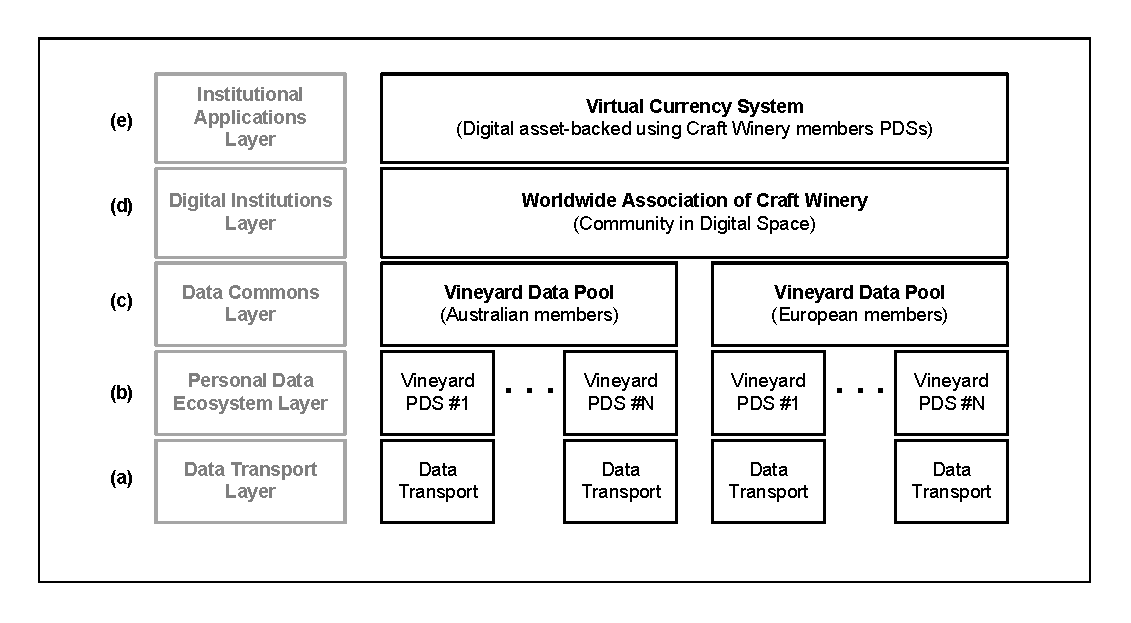
\includegraphics[width=7in]{figure-vineyard-stack}
% where an .eps filename suffix will be assumed under latex, 
% and a .pdf suffix will be assumed for pdflatex; or what has been declared
% via \DeclareGraphicsExtensions.
\caption{Example of a Digital Institution and Application}
\label{fig:vineyard-stack}
\end{figure*}


Figure~\ref{fig:vineyard-stack} attempts to illustrate
the use-case of small craft vineyards around the world
that co-operate and trade among themselves in their
digital institution.  
Here, it is the wine-related trading that is
the institutional ``application'' in this layer.
This application may not be the sole application being
used by the craft winery community.
Another application could be a shared world-wide weather
database specific to the craft winery community.

The point here is that each digital institution
has the freedom to define and self-enforce their
legal trust framework by way of computational law technologies.
Furthermore, as shown in Figure~\ref{fig:vineyard-stack},
the participation of distinct data-pools (as independent
sets of data) allows each local digital community
to establish, manage and govern the usage of theor respective
data pools.
It also allows heterogeneous data -- and therefore more rich data --
to be shared within a global digital community.
Note that Figure~\ref{fig:vineyard-stack} also attempts to illustrate
the use of pools of data (created from personal data stores)
as the basis for creating an asset-backed virtual currency system.






\end{description}



\subsection{A new Paradigm for Digital Institutional Control}


~~\\
~~\\












